\section{Exponential as $f(t)$}
Compute the convolution of an exponential signal $f(t) = e^{at}$ with a rectangular kernel:

\begin{equation}
h(t) = 
\begin{cases} 
1 & \text{for } -T \leq t \leq T \\
0 & \text{otherwise}
\end{cases}
\end{equation}

We will analyze:
\begin{enumerate}
    \item Standard convolution $y(t) = (f*h)(t)$
    \item Modified kernel for $t > 0$
    \item Time-shifted kernel by $\tau_0$
\end{enumerate}

\subsection{Standard Convolution}
\subsubsection{General Solution}
The convolution integral is defined as:

\begin{align}
y(t) &= \int_{-\infty}^{\infty} f(\tau)h(t-\tau)d\tau \\
&= \int_{-\infty}^{\infty} e^{a\tau}h(t-\tau)d\tau
\end{align}

Since $h(t-\tau)$ is non-zero only when $-T \leq t-\tau \leq T$, or equivalently, $t-T \leq \tau \leq t+T$, we can rewrite:

\begin{align}
y(t) &= \int_{t-T}^{t+T} e^{a\tau}d\tau \\
&= \left[ \frac{e^{a\tau}}{a} \right]_{t-T}^{t+T} \quad \text{(for $a \neq 0$)}
\end{align}

Evaluating the integral for $a \neq 0$:

\begin{align}
y(t) &= \frac{e^{a(t+T)}}{a} - \frac{e^{a(t-T)}}{a} \\
&= \frac{e^{at}e^{aT} - e^{at}e^{-aT}}{a} \\
&= \frac{e^{at}(e^{aT} - e^{-aT})}{a} \\
&= \frac{2e^{at}\sinh(aT)}{a}
\end{align}

For the special case when $a = 0$:

\begin{align}
y(t) &= \int_{t-T}^{t+T} e^{0\cdot\tau}d\tau \\
&= \int_{t-T}^{t+T} 1 \, d\tau \\
&= [{\tau}]_{t-T}^{t+T} \\
&= (t+T) - (t-T) \\
&= 2T
\end{align}

\subsubsection{Time Domain Analysis}
The solution is time-invariant - the same form applies for all values of $t$:

\begin{equation}
y(t) = 
\begin{cases}
\frac{2e^{at}\sinh(aT)}{a} & a \neq 0 \\
2T & a = 0
\end{cases}
\end{equation}

For $a > 0$, the output grows exponentially, amplified by the factor $\frac{2\sinh(aT)}{a}$.

For $a < 0$, the output decays exponentially, with the same amplification factor. Here is a plot for different values of 'a'
\begin{figure}[H]
    \centering
    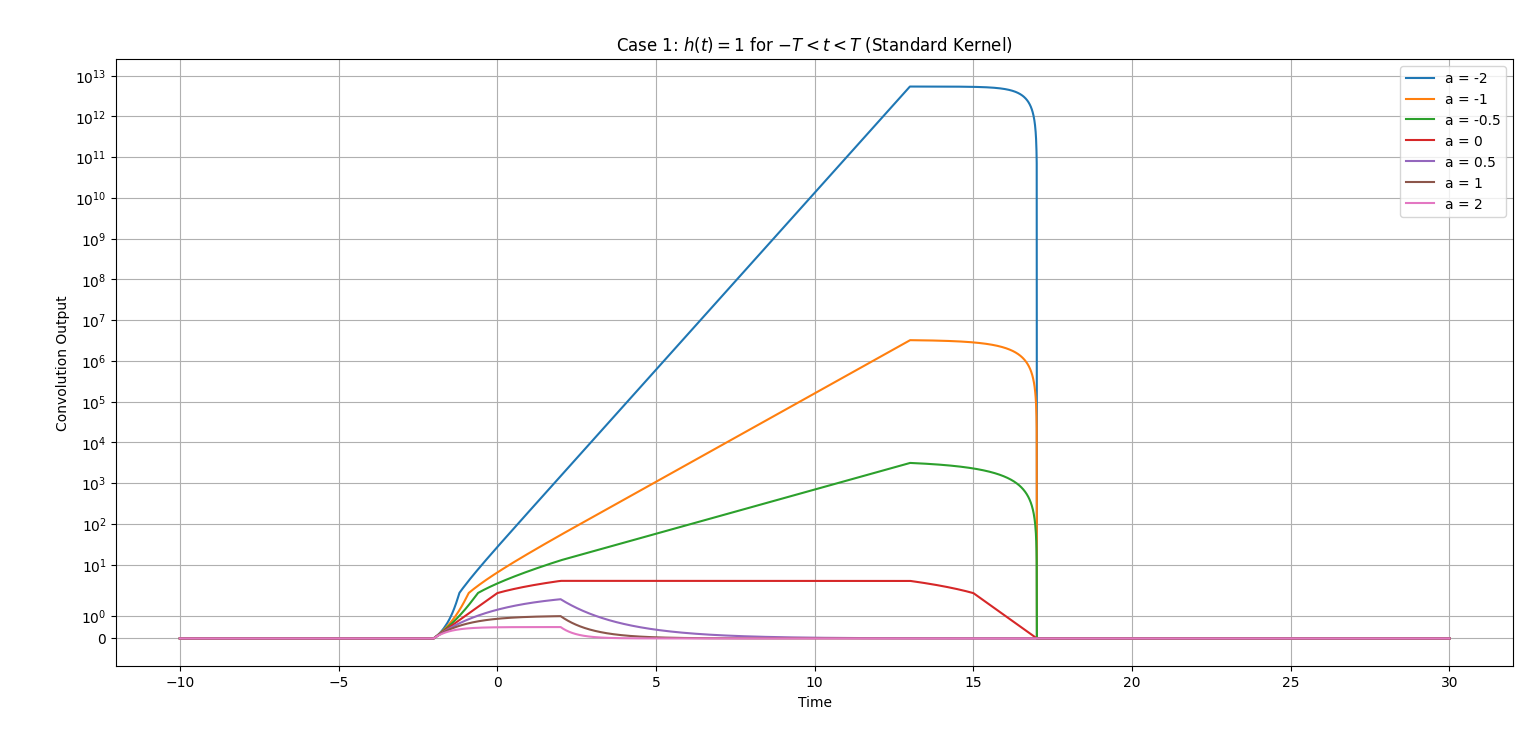
\includegraphics[width=0.8\linewidth]{codes/codes_exp/plotseax/standardkernelvaryinga.png}
    \caption{Varying a}
    \label{fig:enter-label}
\end{figure}
\begin{figure}[H]
    \centering
    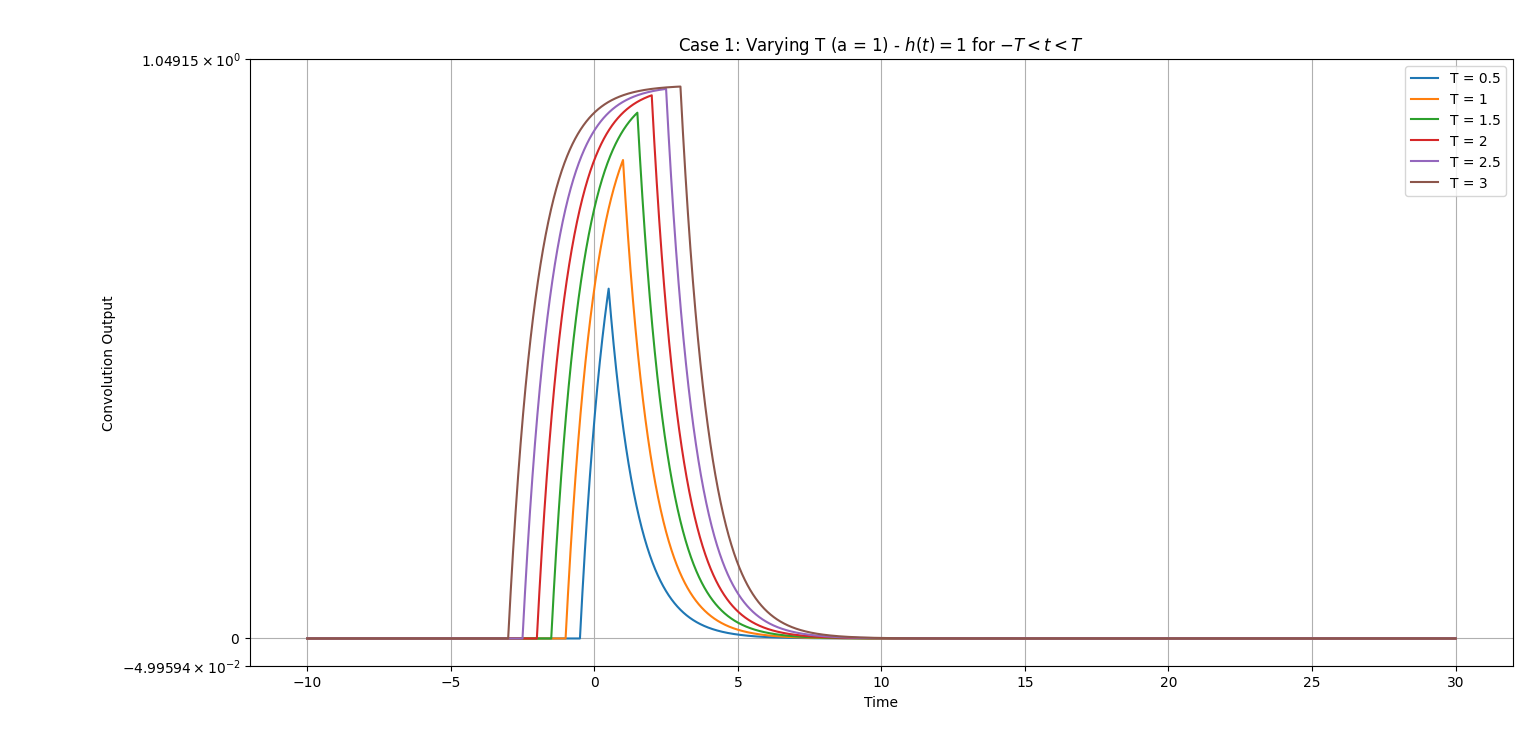
\includegraphics[width=0.8\linewidth]{codes/codes_exp/plotseax/standardkernelcaryingT.png}
    \caption{Varying T}
    \label{fig:enter-label}
\end{figure}

\subsection{Modified Kernel (t $>$ 0)}
\subsubsection{Kernel Definition}
The modified kernel that only considers $t > 0$ is:

\begin{equation}
h_{mod}(t) = 
\begin{cases} 
1 & \text{for } 0 \leq t \leq T \\
0 & \text{otherwise}
\end{cases}
\end{equation}

\subsubsection{Convolution Result}
The convolution integral becomes:

\begin{align}
y(t) &= \int_{-\infty}^{\infty} e^{a\tau}h_{mod}(t-\tau)d\tau
\end{align}

The kernel $h_{mod}(t-\tau)$ is non-zero only when $0 \leq t-\tau \leq T$, or equivalently, $t-T \leq \tau \leq t$.

We also need to consider that $e^{a\tau}$ is defined for all $\tau$. This gives us:

\begin{align}
y(t) &= \int_{t-T}^{t} e^{a\tau}d\tau
\end{align}

However, we must also account for the domain of integration. If $t < 0$, there's no overlap between the kernel and the input. If $0 \leq t < T$, we need to adjust the lower limit.

This gives us three cases:

\begin{enumerate}
    \item \textbf{For $t < 0$:}
    \begin{align}
        y(t) &= 0 \quad \text{(No overlap)}
    \end{align}
    
    \item \textbf{For $0 \leq t \leq T$:}
    \begin{align}
        y(t) &= \int_{0}^{t} e^{a\tau}d\tau \\
        &= \left[ \frac{e^{a\tau}}{a} \right]_{0}^{t} \\
        &= \frac{e^{at} - 1}{a} \quad \text{(for $a \neq 0$)}
    \end{align}
    
    \item \textbf{For $t > T$:}
    \begin{align}
        y(t) &= \int_{t-T}^{t} e^{a\tau}d\tau \\
        &= \left[ \frac{e^{a\tau}}{a} \right]_{t-T}^{t} \\
        &= \frac{e^{at} - e^{a(t-T)}}{a} \\
        &= \frac{e^{at}(1 - e^{-aT})}{a} \quad \text{(for $a \neq 0$)}
    \end{align}
\end{enumerate}

For $a = 0$, the results simplify to:
\begin{align}
y(t) = 
\begin{cases}
0 & t < 0 \\
t & 0 \leq t \leq T \\
T & t > T
\end{cases}
\end{align}
 Here is a plot for different values of 'a'
 \begin{figure}[H]
     \centering
     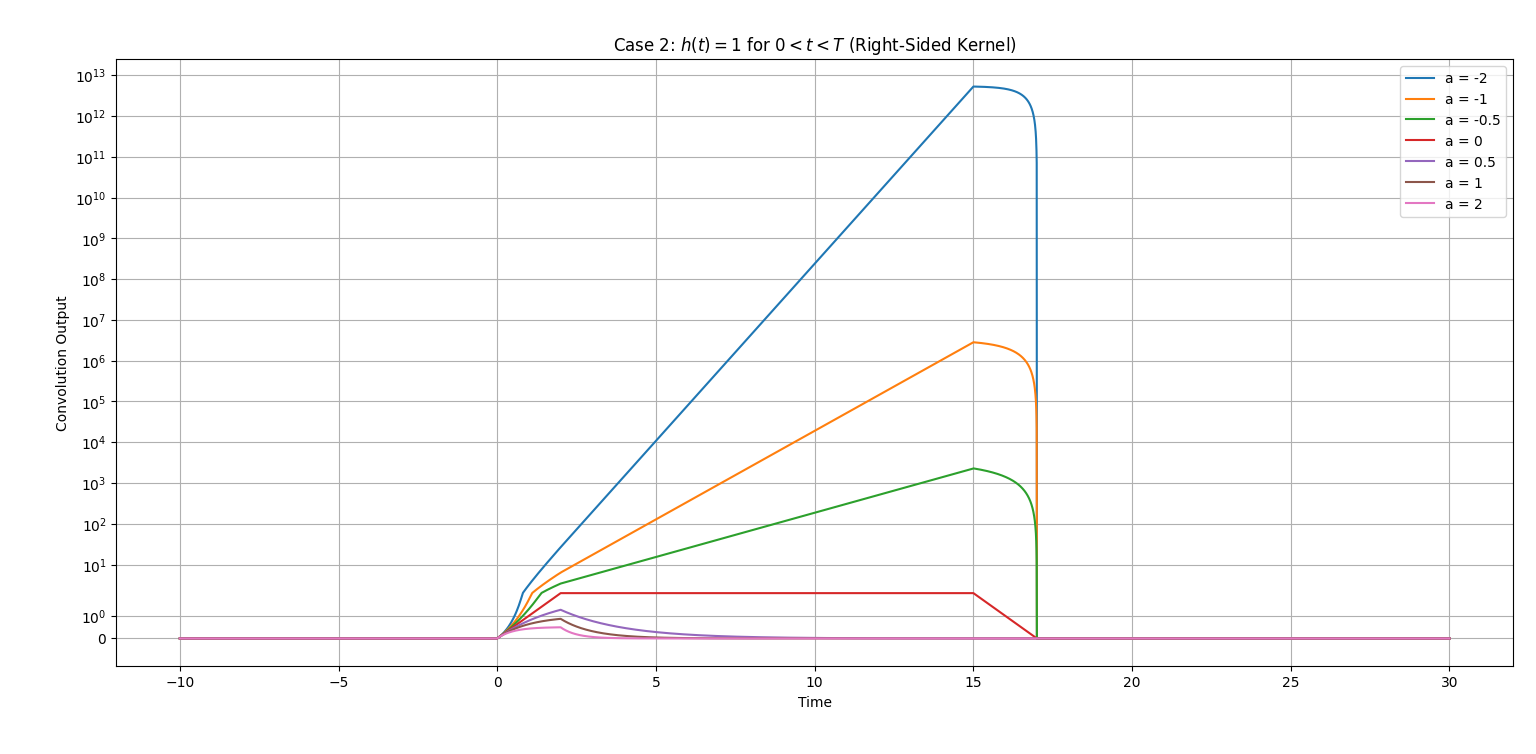
\includegraphics[width=0.8\linewidth]{codes/codes_exp/plotseax/right side kernelvaryinga.png}
     \caption{Varying a}
     \label{fig:enter-label}
 \end{figure}
 Here is a plot showing the variation of T
 \begin{figure}[H]
     \centering
     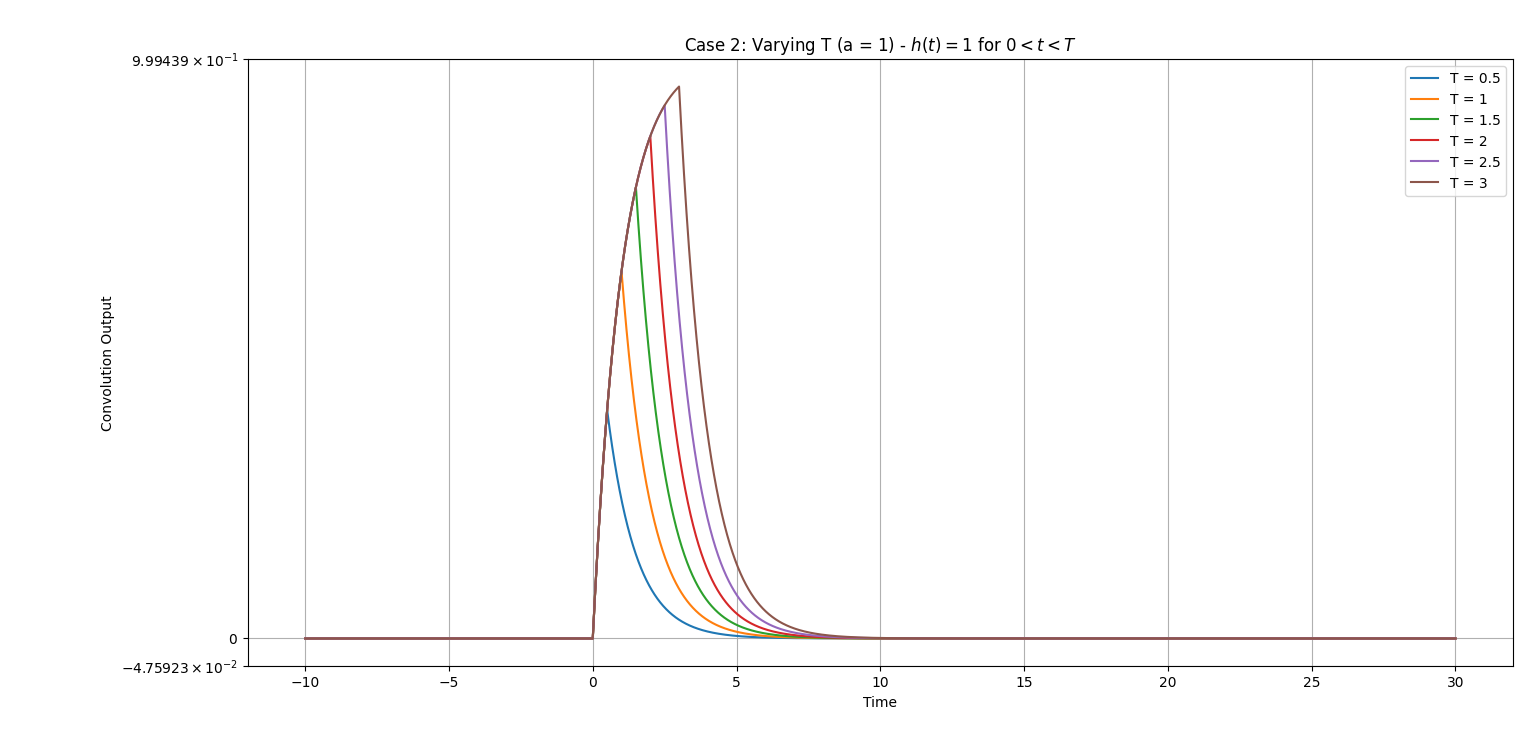
\includegraphics[width=0.8\linewidth]{codes/codes_exp/plotseax/right side kernelvaryingT.png}
     \caption{Varying T}
     \label{fig:enter-label}
 \end{figure}
\subsection{Time-Shifted Kernel}
\subsubsection{Kernel Definition}
The time-shifted rectangular kernel is:

\begin{equation}
h_{shift}(t) = 
\begin{cases} 
1 & \text{for } -T+\tau_0 \leq t \leq T+\tau_0 \\
0 & \text{otherwise}
\end{cases}
\end{equation}

\subsubsection{Convolution Result}
Using the time-shift property of convolution:

\begin{align}
f(t) * h(t-\tau_0) = (f(t) * h(t))_{t \rightarrow t-\tau_0}
\end{align}

Therefore, the convolution with the shifted kernel is simply the original convolution result shifted by $\tau_0$:

\begin{align}
y_{shift}(t) &= y(t-\tau_0) \\
&= \frac{2e^{a(t-\tau_0)}\sinh(aT)}{a} \quad \text{(for $a \neq 0$)} \\
&= \frac{2e^{at}e^{-a\tau_0}\sinh(aT)}{a} \\
&= e^{-a\tau_0} \cdot \frac{2e^{at}\sinh(aT)}{a}
\end{align}

For $a = 0$:
\begin{align}
y_{shift}(t) = 2T
\end{align}
Here are a few plots to demonstrate the result
\begin{figure}[H]
    \centering
    { 
    \subfloat[a=0]{
    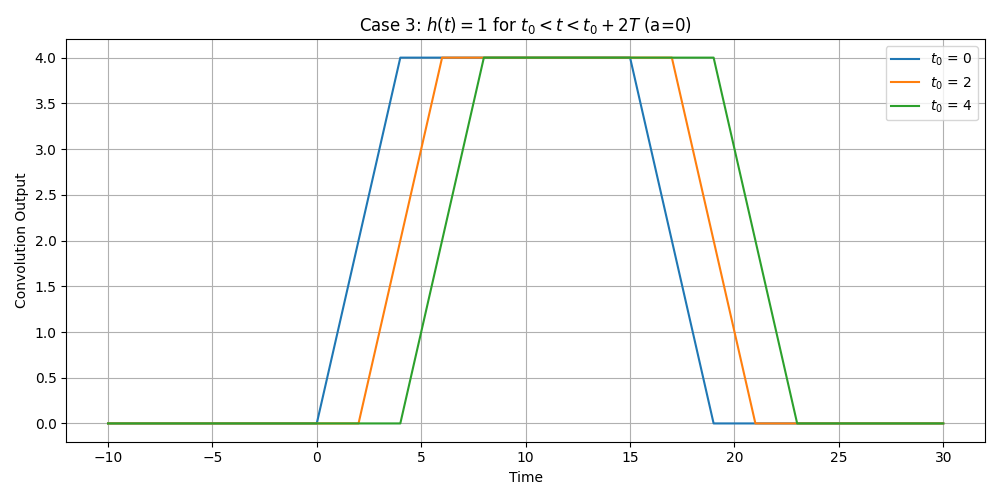
\includegraphics[width=0.45\textwidth]{codes/codes_exp/plotseax/case3a=0.png}
    
    }
    \subfloat[a=-1]{
        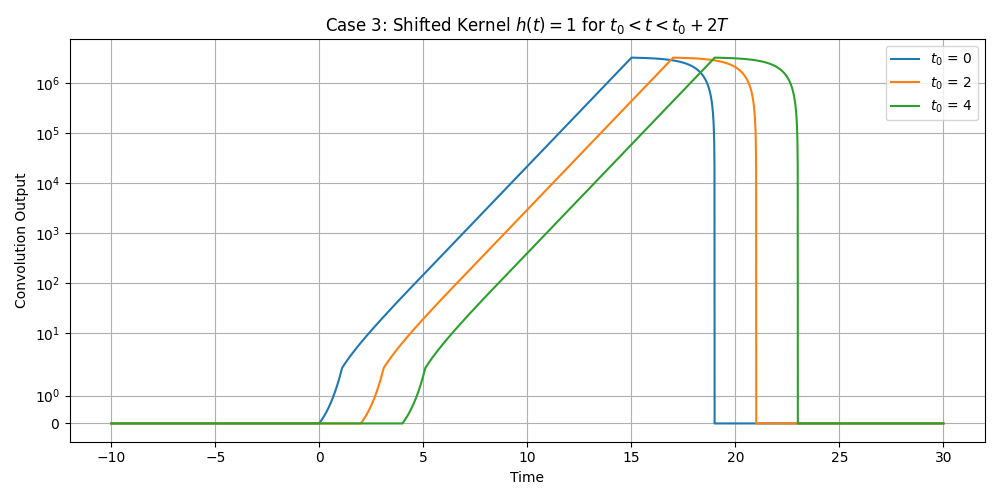
\includegraphics[width=0.45\textwidth]{codes/codes_exp/plotseax/case3a=-1.png}
    }
    }
\end{figure}
\begin{figure}[H]
    \centering
    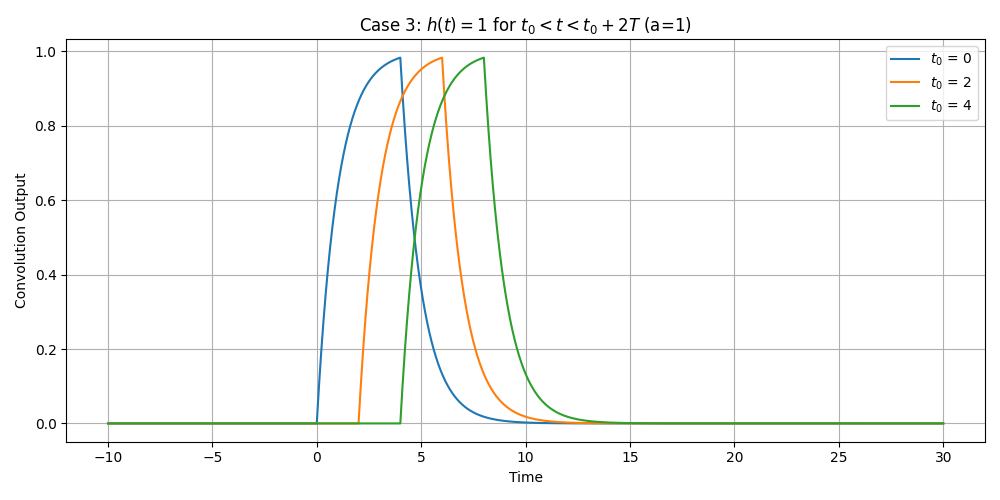
\includegraphics[width=0.7\linewidth]{codes/codes_exp/plotseax/case3a=1.png}
    \caption{a=1}
    \label{fig:enter-label}
\end{figure}
\subsection{Conclusion}
\begin{itemize}
    \item \textbf{Standard Convolution:} The exponential input produces a scaled exponential output, with the scaling factor depending on the kernel width $T$ and the exponential parameter $a$.
    
    \item \textbf{Kernel Width Effect:} The parameter $T$ controls the amplification via the $\sinh(aT)$ term. Larger values of $T$ result in greater amplification.
    
    \item \textbf{Time-Shift Effect:} A time-shift of $\tau_0$ introduces a pure delay in the output, equivalent to multiplying the original output by $e^{-a\tau_0}$.
    
    \item \textbf{Causal Modification:} Making the kernel causal (only for $t > 0$) changes the initial conditions and creates a time-varying response that depends on the region of $t$.
    
    \item \textbf{Special Case:} When $a = 0$ (constant input), the output is simply proportional to the width of the kernel, demonstrating the averaging property of convolution.
\end{itemize}

This analysis provides insight into how convolution with a rectangular kernel affects exponential signals, which is fundamental in understanding linear time-invariant systems.
\subsubsection{Time-Invariance Analysis}
To prove that our system is time-invariant, we need to show that a time-shifted input results in an equally time-shifted output. 

Let's consider our original input $f(t) = e^{at}$ with output $y(t) = \frac{2e^{at}\sinh(aT)}{a}$ for $a \neq 0$.

If we time-shift the input by $t_0$ to get $f'(t) = f(t-t_0) = e^{a(t-t_0)} = e^{at}e^{-at_0}$, the corresponding output would be:

\begin{align}
y'(t) &= \int_{-\infty}^{\infty} f'(\tau)h(t-\tau)d\tau \\
&= \int_{-\infty}^{\infty} e^{a(\tau-t_0)}h(t-\tau)d\tau \\
&= e^{-at_0}\int_{-\infty}^{\infty} e^{a\tau}h(t-\tau)d\tau \\
&= e^{-at_0} \cdot y(t)
\end{align}

However, the time-shifted output of the original system would be:
\begin{align}
y(t-t_0) &= \frac{2e^{a(t-t_0)}\sinh(aT)}{a} \\
&= \frac{2e^{at}e^{-at_0}\sinh(aT)}{a} \\
&= e^{-at_0} \cdot \frac{2e^{at}\sinh(aT)}{a} \\
&= e^{-at_0} \cdot y(t)
\end{align}

Since $y'(t) = y(t-t_0)$, this confirms that the system is time-invariant.

The system is time-invariant because:
\begin{itemize}
    \item The rectangular kernel $h(t)$ depends only on the relative time difference $(t-\tau)$, not on absolute time.
    \item The convolution operation itself preserves time-invariance.
    \item The system's response at any time $t$ depends only on the input over the interval $[t-T, t+T]$, regardless of when this interval occurs.
    \item The mathematical form of the output maintains the same structure regardless of time shifts in the input.
\end{itemize}

This time-invariance property is fundamental to linear systems theory and allows us to analyze the system using frequency domain techniques.
